\chapter{Mathematical definitions}\label{ch:math_definitions}

\section{Graph theory}

Standard definitions of relevant concepts from graph theory, based mostly on \textsl{A first course in network theory}~\cite{Estrada2017}.

\begin{definition}[Graph]
    Let $V$ be a finite set of $n$ nodes (or vertices), and let $E \subseteq V \times V$ be a set of edges.\\
    A \textbf{graph} $G$ is a pair $(V, E)$.\\
    $V$ is the \textbf{node set} of $G$, and $E$ is the \textbf{edge set} of $G$.
\end{definition}

\begin{definition}[Graph properties]
    \begin{itemize}[leftmargin=*]
        \item $G$ is \textbf{reflexive} iff $\forall v \in V.\ (v, v) \in E$
        \item $G$ is \textbf{anti-reflexive} iff $\forall v \in V.\ (v, v) \notin E$
        \item $G$ is \textbf{undirected} (or equally \textbf{symmetric}) iff $\forall v_1, v_2 \in V.\ (v_1, v_2) \in E \Rightarrow (v_2, v_1) \in E$
        \item $G$ is \textbf{directed} iff it is not undirected
        \item $G$ is a \textbf{simple graph} iff it is undirected and anti-reflexive
    \end{itemize}
\end{definition}

\begin{definition}[Relations on graphs]
    \begin{itemize}[leftmargin=*]
        \item $G' = (V', E')$ is a \textbf{subgraph} of $G = (V, E)$ iff $V' \subseteq V$ and $E' \subseteq E$
        \item Let $G_1 = (V_1, E_1)$ and $G_2 = (v_2, E_2)$, then $G_1 \cup G_2 = (V_1 \cup V_2, E_1 \cup E_2)$ is the \textbf{union} of the two graphs, and $G_1 \cap G_2 = (V_1 {\cap} V_2, E_1 {\cap} E_2)$ is the \textbf{intersection} of the two graphs.
    \end{itemize}
\end{definition}

\begin{definition_with_break}[Node adjacency]
    \begin{itemize}[leftmargin=*]
        \item In an undirected graph, $v_1$ is \textbf{adjacent} to $v_2$ iff $(v_1, v_2) \in E$
        \item A \textbf{loop} is an edge of the form $(v, v)$.
        Note that simple graphs have no loops.
        \item Define $\deg^-(v) = \left\lvert \Set{v' \in V}{(v', v) \in E} \right\rvert$ to be the \textbf{indegree} of $v$, and $\deg^+(v) = \left\lvert \Set{v' \in V}{(v, v') \in E} \right\rvert$ to be the \textbf{outdegree} of $v$, in other words, the number of incoming and outcoming edges, respectively.
        If the graph is undirected, then $\deg^-(v) = \deg^+(v) = \deg(v)$ is called \textbf{degree}.
        \item For $G = (V, E)$ with $V = \integersto{n}$, define $A = (a_{ij})$ to be the \textbf{adjacency matrix} of $G$ where
        \[ a_{ij} = \begin{cases}
                        1, & \textnormal{if}\ (i, j) \in E \\
                        0, & \textnormal{if}\ (i, j) \notin E
        \end{cases} \]
        for $1 \leq i, j \leq n$.

        Note that adjacency matrix of undirected graph is symmetric.
    \end{itemize}
\end{definition_with_break}

\begin{definition}[Connectedness]
    \begin{itemize}[leftmargin=*]
        \item $u, v$ are \textbf{connected nodes} is there exists a path between $u, v$ in $G$, i.e. if $(A^k)_{uv} = 1$ for some $k\in \mathbb{N}$.
        \item $G = (V, E)$ is \textbf{connected graph} if $\forall v_1, v_2 \in V. v_1, v_2$ are connected nodes.
        \item A subgraph $G' \subseteq G$ is a \textbf{(connected) component} iff $G'$ is a maximal connected subgraph of $G$.

        Note that all components of a graph are disjoint, therefore each node belongs to exactly one component.
    \end{itemize}

    \item A \textbf{giant component} of a graph is a single component that has more nodes than any other component of the graph.

    Note that a giant component may not exist if more components have the maximum number of nodes.
\end{definition}


\section{Ranking}

These definitions precede those in \cref{sec:ranking}.

\begin{definition}[Partial order]
    A binary relation $\sqsubseteq$ on some set $P$ is a \textbf{partial order} iff it is antisymmetric preorder, i.e.:
    \begin{itemize}
        \item $\forall a, b \in P.\ a \sqsubseteq a$ \tabto{7.3cm}(reflexivity)
        \item $\forall a, b, c \in P.\ (a \sqsubseteq b \wedge b \sqsubseteq c) \implies a \sqsubseteq c$ \tabto{7.3cm}(transitivity)
        \item $\forall a, b \in P.\ (a \sqsubseteq b \wedge b \sqsubseteq a) \implies a = b$ \tabto{7.3cm}(antisymmetry)
    \end{itemize}
\end{definition}

\begin{definition}[Total order]
    A binary relation $\sqsubseteq$ on some set $P$ is a \textbf{total order} iff it is a partial order and a connex relation, i.e.:
    \begin{itemize}
        \item $\forall a, b, c \in P.\ (a \sqsubseteq b \wedge b \sqsubseteq c) \implies a \sqsubseteq c$ \tabto{7.3cm}(transitivity)
        \item $\forall a, b \in P.\ (a \sqsubseteq b \wedge b \sqsubseteq a) \implies a = b$ \tabto{7.3cm}(antisymmetry)
        \item $\forall a, b \in P.\ a \sqsubseteq b \vee b \sqsubseteq a$ \tabto{7.3cm}(connexity, implies reflexivity)
    \end{itemize}
\end{definition}



\chapter{Kotlin figures}\label{ch:appendix_kotlin_figures}
% Kotlin architecture
% Program figures
% Project figures

\begin{figure}
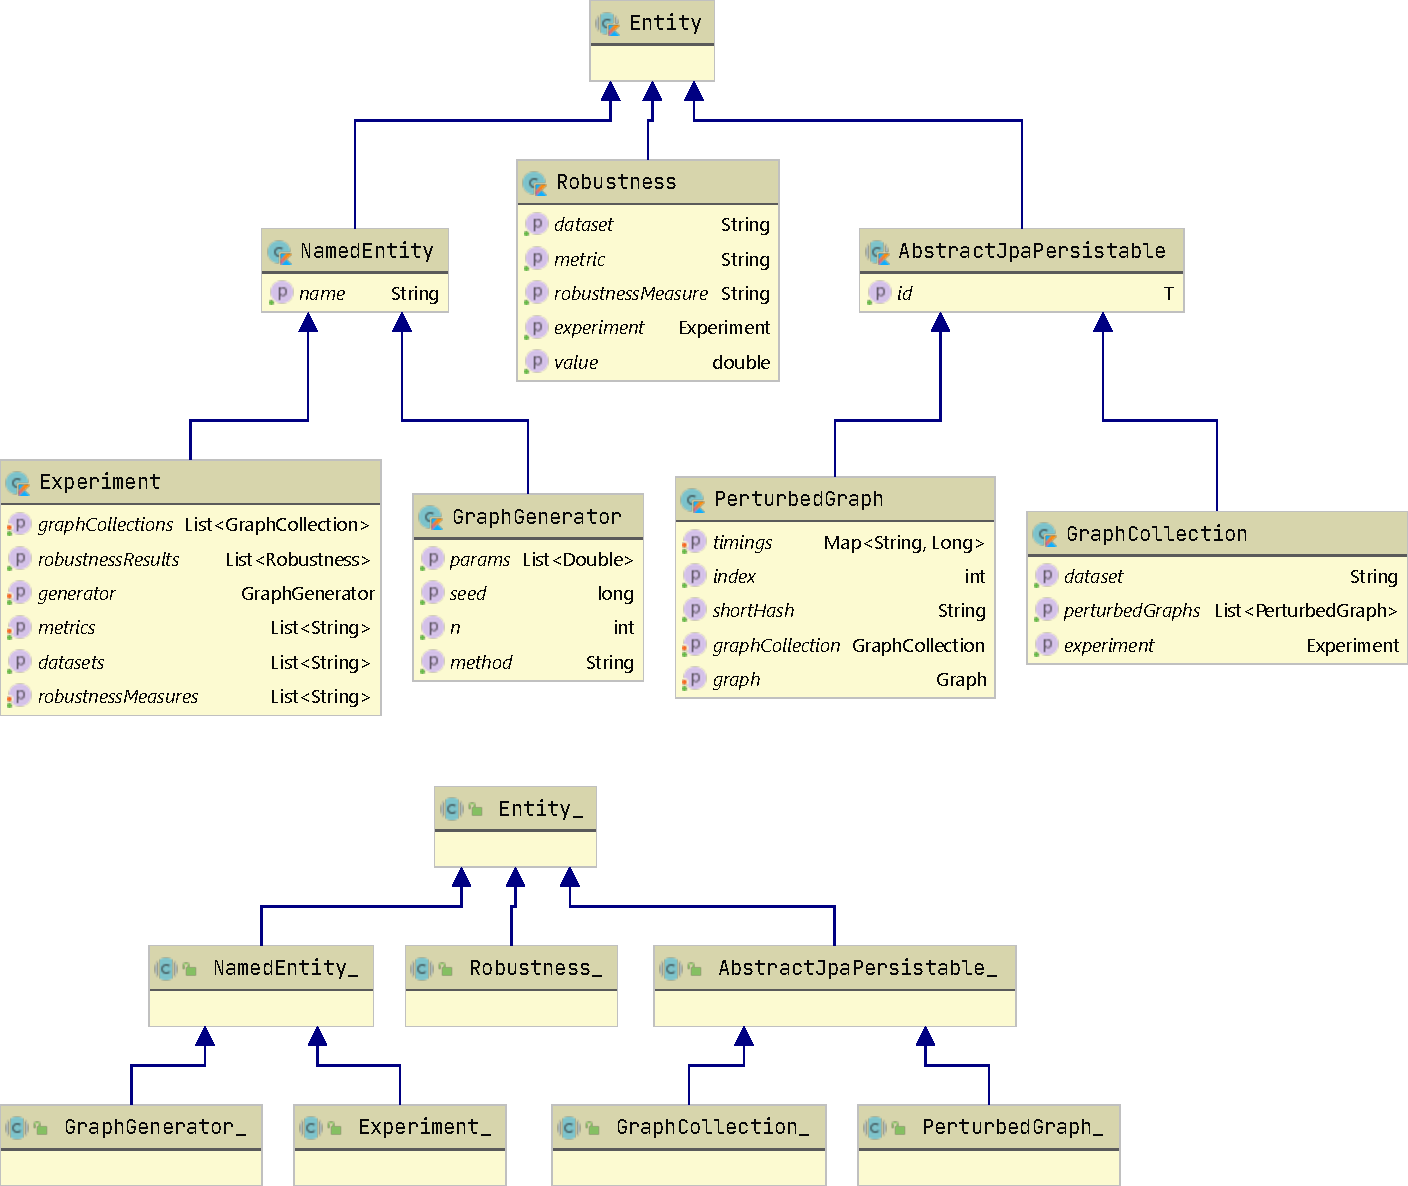
\includegraphics[width=\linewidth]{data_model_classes_diagram.pdf}
\caption{Inheritance hierarchy of the (Kotlin) classes underlying the persistence model presented in \autoref{fig:data_model_diagram}.
The arrows indicate \textsl{inheritance} (``is a'') relationships between classes.}
\label{fig:data_model_classes_diagram}
\end{figure}


\begin{figure}
    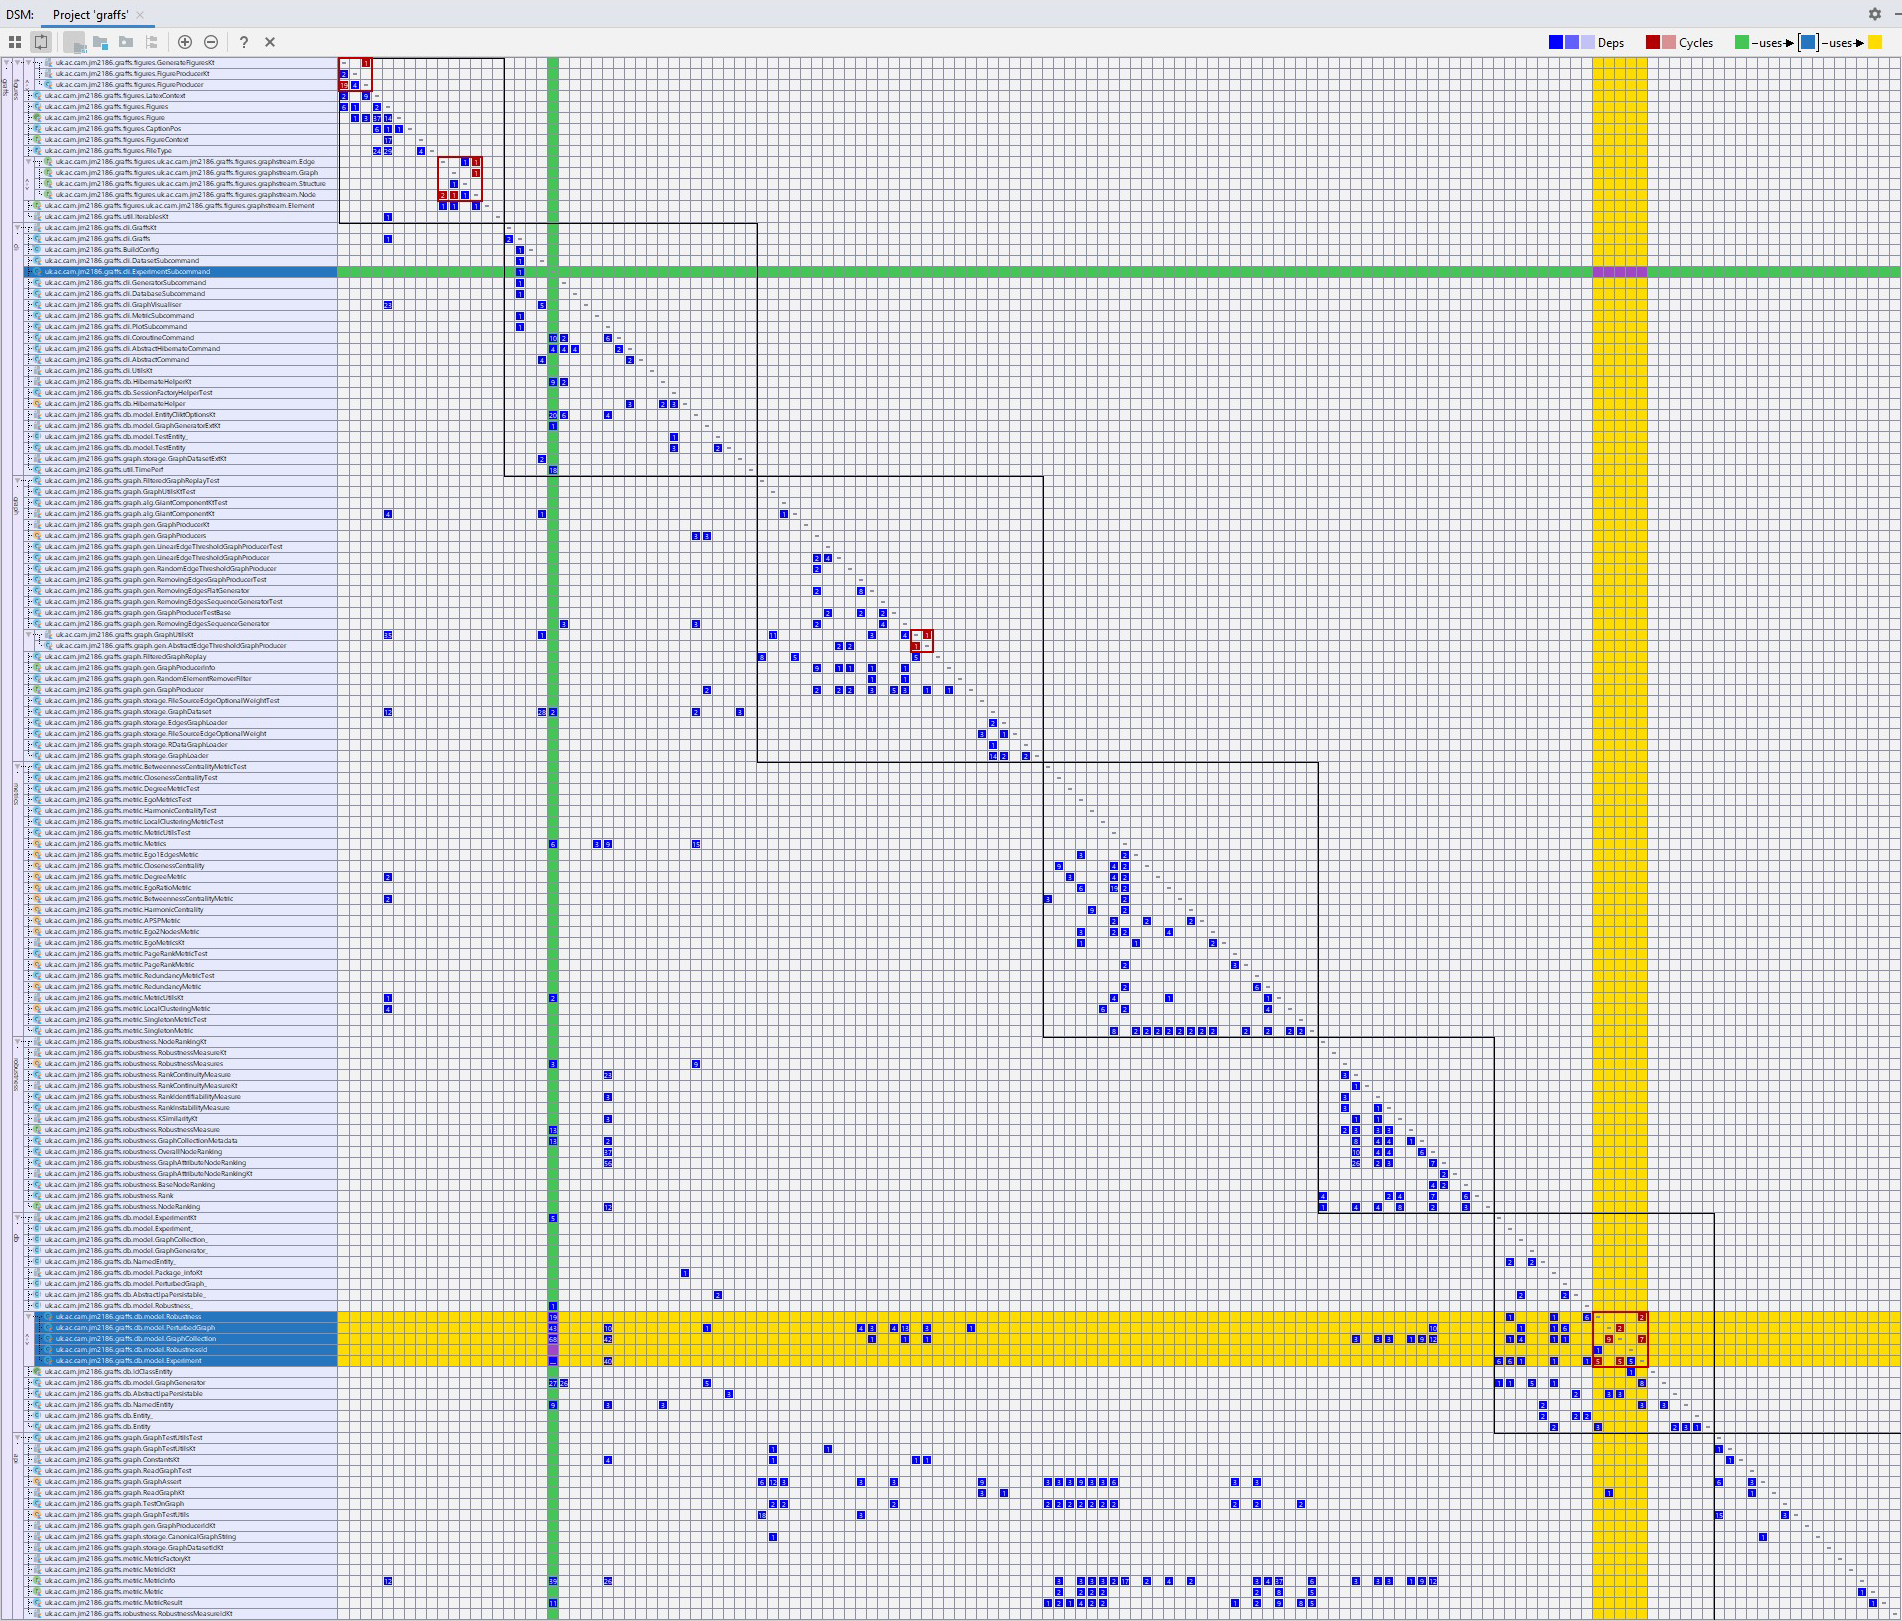
\includegraphics[width=\linewidth]{classes_dependency_matric.png}
    \caption{Dependency matrix between Kotlin files of \graffs (excluding tests), visualised by the IntelliJ IDEA editor.
    Each of the 7 groups corresponds to a module, namely: \texttt{figures}, \texttt{cli}, \texttt{graph}, \texttt{metric}, \texttt{robustness}, \texttt{db}, \texttt{api}.
    Cell in $i$-th row from the top and $j$-th column from the left corresponds to the dependency of $j$-th file on $i$-th file.
    Modules and files are ordered from more dependent (top) to less dependent (bottom).}
    \label{fig:classes_dependency_matrix}
    \footnotesize\justify\vspace{-0.4\baselineskip}
    The highlighted rows and columns show the directed dependency of the \texttt{ExperimentSubcommand} class (green), which provides the \texttt{graffs experiment} command-line subcommands, on the 5 JPA entity classes from \cref{fig:data_model_classes_diagram} (yellow).
\end{figure}


\clearpage

\lstinputlisting[label={lst:jpa_typed_query}, linerange=jpa_typed_query0-jpa_typed_query1, caption={A toy example of using typed Java Persistence API queries. Note the \texttt{Experiment\_} metamodel class generated from the \texttt{Experiment} entity by Hibernate, with (meta)fields corresponding to entities' fields.}, float, language=Kotlin]{listings.kts}

\lstinputlisting[label={lst:hibernate_load_entity}, linerange=hibernate_load_entity0-hibernate_load_entity1, caption={A toy example of Hibernate loading and persisting an \texttt{Experiment} object.}, float, language=Kotlin]{listings.kts}

\lstinputlisting[label={lst:graffs_cli_examples}, caption={A demonstration of the command-line help text of some subcommands, printed by \graffs}, float, basicstyle=\ttfamily\color{black}\fontsize{8pt}{8pt}\selectfont,]{graffs-help.txt}


\chapter{Robustness results}\label{ch:appendix_results}

\begin{table}[H]
\setlength{\tabcolsep}{5pt}\renewcommand{\arraystretch}{1}
\caption{RankContinuity of 7 metrics on 8 datasets (experiments \texttt{random-edges} and \texttt{unscored})}
\label{tab:robustness-continuity}
\scalebox{1}{
\begin{tabular}{|p{40mm}|ccc|ccccc|}
\toprule
{\small \textbf{RankContinuity}} & {\footnotesize \texttt{pvivax}} & {\footnotesize \texttt{ecoli}} & {\footnotesize \texttt{yeast}} & {\footnotesize \texttt{airports}} & {\footnotesize \texttt{collab}} & {\footnotesize \texttt{citation}} & {\footnotesize \texttt{facebook}} & {\footnotesize \texttt{internet}} \\
\midrule
                     Betweenness &                   {\small 1.00} &                  {\small 1.00} &                  {\small 1.00} &                     {\small 1.00} &                   {\small 0.70} &                     {\small 1.00} &                     {\small 0.83} &                     {\small 1.00} \\
                          Degree &                   {\small 1.00} &                  {\small 1.00} &                  {\small 1.00} &                     {\small 1.00} &                   {\small 1.00} &                     {\small 1.00} &                     {\small 1.00} &                     {\small 1.00} \\
                       Ego1Edges &                   {\small 1.00} &                  {\small 1.00} &                  {\small 1.00} &                     {\small 1.00} &                   {\small 1.00} &                     {\small 1.00} &                     {\small 1.00} &                     {\small 1.00} \\
                       Ego2Nodes &                   {\small 1.00} &                  {\small 1.00} &                  {\small 1.00} &                     {\small 1.00} &                   {\small 1.00} &                     {\small 1.00} &                     {\small 0.97} &                     {\small 1.00} \\
                 LocalClustering &                   {\small 0.23} &                  {\small 0.10} &                  {\small 0.07} &                     {\small 0.60} &                   {\small 0.33} &                     {\small 0.00} &                     {\small 0.07} &                     {\small 1.00} \\
                        PageRank &                   {\small 1.00} &                  {\small 1.00} &                  {\small 1.00} &                     {\small 1.00} &                   {\small 1.00} &                     {\small 1.00} &                     {\small 1.00} &                     {\small 1.00} \\
                      Redundancy &                   {\small 0.87} &                  {\small 1.00} &                  {\small 1.00} &                     {\small 1.00} &                   {\small 1.00} &                     {\small 0.73} &                     {\small 1.00} &                     {\small 1.00} \\
\bottomrule
\end{tabular}
}
\vspace*{2mm}
\caption{RankIdentifiability of 7 metrics on 8 datasets (experiments \texttt{random-edges} and \texttt{unscored})}
\label{tab:robustness-identifiability}
\scalebox{1}{
\begin{tabular}{|p{40mm}|ccc|ccccc|}
\toprule
{\small \textbf{RankIdentifiability}} & {\footnotesize \texttt{pvivax}} & {\footnotesize \texttt{ecoli}} & {\footnotesize \texttt{yeast}} & {\footnotesize \texttt{airports}} & {\footnotesize \texttt{collab}} & {\footnotesize \texttt{citation}} & {\footnotesize \texttt{facebook}} & {\footnotesize \texttt{internet}} \\
\midrule
                          Betweenness &                   {\small 0.93} &                  {\small 0.94} &                  {\small 0.94} &                     {\small 0.97} &                   {\small 0.81} &                     {\small 0.91} &                     {\small 0.83} &                     {\small 1.00} \\
                               Degree &                   {\small 0.99} &                  {\small 1.00} &                  {\small 0.99} &                     {\small 1.00} &                   {\small 0.97} &                     {\small 1.00} &                     {\small 0.98} &                     {\small 1.00} \\
                            Ego1Edges &                   {\small 0.94} &                  {\small 1.00} &                  {\small 0.95} &                     {\small 1.00} &                   {\small 0.98} &                     {\small 0.97} &                     {\small 0.98} &                     {\small 1.00} \\
                            Ego2Nodes &                   {\small 0.94} &                  {\small 0.97} &                  {\small 0.74} &                     {\small 0.92} &                   {\small 0.82} &                     {\small 0.86} &                     {\small 0.35} &                     {\small 1.00} \\
                      LocalClustering &                   {\small 0.09} &                  {\small 0.13} &                  {\small 0.34} &                     {\small 0.14} &                   {\small 0.29} &                     {\small 0.13} &                     {\small 0.07} &                     {\small 1.00} \\
                             PageRank &                   {\small 0.99} &                  {\small 0.97} &                  {\small 0.96} &                     {\small 1.00} &                   {\small 0.89} &                     {\small 0.99} &                     {\small 0.94} &                     {\small 1.00} \\
                           Redundancy &                   {\small 0.85} &                  {\small 0.98} &                  {\small 0.98} &                     {\small 0.92} &                   {\small 0.97} &                     {\small 0.80} &                     {\small 0.99} &                     {\small 1.00} \\
\bottomrule
\end{tabular}
}
\vspace*{2mm}
\caption{RankInstability of 7 metrics on 8 datasets (experiments \texttt{random-edges} and \texttt{unscored})}
\label{tab:robustness-instability}
\scalebox{1}{
\begin{tabular}{|p{40mm}|ccc|ccccc|}
\toprule
{\small \textbf{RankInstability}} & {\footnotesize \texttt{pvivax}} & {\footnotesize \texttt{ecoli}} & {\footnotesize \texttt{yeast}} & {\footnotesize \texttt{airports}} & {\footnotesize \texttt{collab}} & {\footnotesize \texttt{citation}} & {\footnotesize \texttt{facebook}} & {\footnotesize \texttt{internet}} \\
\midrule
                      Betweenness &                   {\small 0.00} &                  {\small 0.00} &                  {\small 0.01} &                     {\small 0.00} &                   {\small 0.02} &                     {\small 0.01} &                     {\small 0.01} &                     {\small 0.00} \\
                           Degree &                   {\small 0.00} &                  {\small 0.00} &                  {\small 0.00} &                     {\small 0.00} &                   {\small 0.01} &                     {\small 0.00} &                     {\small 0.01} &                     {\small 0.00} \\
                        Ego1Edges &                   {\small 0.01} &                  {\small 0.01} &                  {\small 0.01} &                     {\small 0.01} &                   {\small 0.01} &                     {\small 0.00} &                     {\small 0.01} &                     {\small 0.00} \\
                        Ego2Nodes &                   {\small 0.01} &                  {\small 0.00} &                  {\small 0.02} &                     {\small 0.02} &                   {\small 0.01} &                     {\small 0.01} &                     {\small 0.05} &                     {\small 0.00} \\
                  LocalClustering &                   {\small 0.04} &                  {\small 0.08} &                  {\small 0.04} &                     {\small 0.12} &                   {\small 0.16} &                     {\small 0.09} &                     {\small 0.12} &                     {\small 0.00} \\
                         PageRank &                   {\small 0.00} &                  {\small 0.00} &                  {\small 0.00} &                     {\small 0.00} &                   {\small 0.01} &                     {\small 0.00} &                     {\small 0.01} &                     {\small 0.00} \\
                       Redundancy &                   {\small 0.02} &                  {\small 0.01} &                  {\small 0.01} &                     {\small 0.02} &                   {\small 0.01} &                     {\small 0.01} &                     {\small 0.01} &                     {\small 0.00} \\
\bottomrule
\end{tabular}
}
\end{table}

